\documentclass[9pt,twocolumn]{extarticle}

\usepackage[utf8]{inputenc}
\usepackage{newpxtext} % An improved version of the Palantino font...
\usepackage{newpxmath} % ...and its math version.
\usepackage{authblk}   % Use author blocks.
\usepackage[top=2cm,bottom=2.5cm,left=2cm,right=2cm]{geometry}
\usepackage{balance}
\usepackage{tikz}
\usepackage{xspace} % For reasonable spacing in custom commands.
\usepackage{xcolor} % For colourful links.
\usepackage[backend=biber,style=alphabetic,backref=true,maxnames=20,urldate=long]{biblatex}
\usepackage{hyperref} % For clickable links.
\usepackage[l2tabu, orthodox]{nag}
\usepackage{subcaption}

\setlength{\columnsep}{0.7CM}

\addbibresource{paper.bib}

\definecolor{darkblue}{rgb}{0.1,0.1,0.4}

\newcommand{\ie}{{\it i.e.}\xspace}
\newcommand{\eg}{{\it e.g.}\xspace}
\newcommand{\ea}{{\it et al.}\xspace}
\newcommand{\etc}{{\it etc.}\xspace}
\newcommand{\aka}{a.k.a.\xspace}
\newcommand{\first}{(\emph{i})\xspace}
\newcommand{\second}{(\emph{ii})\xspace}
\newcommand{\third}{(\emph{iii})\xspace}
\newcommand{\fourth}{(\emph{iv})\xspace}
\newcommand{\fifth}{(\emph{v})\xspace}

\hypersetup{
	pdftitle={How do Tor users interact with onion services?},
	pdfauthor={},
	pdfkeywords={},
	colorlinks=true,
	urlcolor=darkblue,
	linkcolor=darkblue,
	citecolor=darkblue
}

\renewcommand*{\bibfont}{\small}

\title{
    {\Huge \textbf{How do Tor users interact with onion services?}}
}

\author{}

\begin{document}

\maketitle

\begin{abstract}
The abstract goes here.
\end{abstract}


\section{Introduction}
\label{sec:introduction}

Online anonymity is typically synonymous with \emph{client anonymity}; VPNs
promise to disguise one's IP address, An equally pressing requirement can be
\emph{server anonymity} when the operator of a site is facing harassment or legal
repercussions.  Decoupling a server's content from the identity of its operator
can mitigate these issues.  Several systems implement various flavours of server
anonymity, including I2P, Freenet, and X, but in this work we focus on Tor's
onion services.

The Tor anonymity network is primarily known as a tool that enables client
anonymity, \ie, it allows users who download the project's Tor Browser to
browse the web anonymously~\cite{Dingledine2004a}.  In addition to client
anonymity, Tor provides server anonymity in the form of onion services (\aka
hidden services) which allow operators to expose a TCP service over the Tor
network while hiding its IP address.

Onion services have grown substantially over the last years, both in the number
of services and users.  As of May 2017, The Tor Project's statistics show that
more than 50,000 onion services are online each day, relaying more than 750 MBps
of network traffic.  Not all of these services host web sites---other use cases
such as meta data-free messaging~\cite{ricochet} and file
sharing~\cite{onionshare} have emerged as well.  Learning the number of onion
service users is more challenging.  In 2016, Facebook reported that more than
one million users logged into their onion service over a one month
period~\cite{facebook-users}.
RFC~\cite{rfc7686}

Past usability research focused on Tor Browser~\cite{Clark2007a,Norcie2014a}
and Tor's censorship circumvention~\cite{Fifield2015a}.  The usability of onion
services remains mostly unexplored.

The most salient aspect of onion services is their peculiar domain names.
Being derived from RSA public keys, they consist of random Base32 characters
such as the following three examples.

{\footnotesize
\begin{verbatim}
6hylx55pr5dnod4t.onion
ke33kjltp3twmcwq.onion
4v4ndsnrjekbfhij.onion
\end{verbatim}
}

Onion domains are random, very difficult to remember, and cumbersome to work
with.  The next generation of onion services exacerbates this problem by
employing domains consisting of 54 (instead of sixteen) Base32-encoded
characters, giving them the following format:

{\footnotesize
\begin{verbatim}
lfels7g3rbceenuuqmpsz45z3lswakqf56n5i3bvqhc22d5rrszzwd.onion
llamanymityx4fi3l6x2gyzmtmgxjyqyorj9qsb5r543izcwymlead.onion
odmmeotgcfx65l5hn6ejkaruvai222vs7o7tmtllszqk5xbysolfdd.onion
\end{verbatim}
}

Properties that we take for granted in the non-onion web are not present in the
onion web.  The usability of onion services differs from ordinary websites in
the following aspects that we are trying to capture in our survey.  The first
issue is \emph{accessibility}.  Onion services are only accessible over Tor for
full client anonymity.\footnote{Services such as Tor2web allow normal web
clients to access onion services but that means that users give up client
anonymity~\cite{tor2web}.} The next issue is onion service \emph{discovery}.
It is difficult to learn about new onion sites.  There is no central directory,
and---unlike the web---onion sites do not link to each other
much~\cite{Griffith2017a}.  However, search engines such as ahmia.fi and
onion.link are a beginning.  Once users learn about new onion service, their
\emph{domain format} makes it difficult to memorize them.  Perhaps the most
salient idiosyncrasy of onion domains is that they are generated randomly.  As
a result, onion domains are difficult to memorize and recognize, forcing users
to handle them differently than normal websites.  Browsing onion sites may feel
clunky because of \emph{latency}---the number of hops in between Tor user and
onion service is causing tangible communication latency that many users may not
be willing to tolerate.

To date, only anecdotal evidence exists on how people interact with onion
services.  In this work we seek to fill this gap by administering a survey
designed to answer the following research questions: \emph{How do Tor users
interact with onion services?}  An answer to this research question allows us
to both create more usable anonymity systems and build these systems in a way
that semantic attacks such as phishing are exacerbated.\footnote{Downs \ea
distinguish between physical (\ie targeting physical infrastructure),
syntactic (\ie targeting software), and semantic (\ie targeting humans)
attacks~\cite[\S~1]{Downs2006a}.}  In particular, we seek to answer the
following three aspects:

%%%
In this paper, we answer our research question by conducting a survey.
We seek to inform X and Y to do Z better.
%%%

\begin{itemize}
    \item What is the expectation of privacy when people use Tor Browser in
        general and onion sites in particular?
    \item What is the security/usability trade-off of vanity onion domains?
    \item Do people handle onion domains differently than normal domains?
\end{itemize}

The rest of this paper is structured as follows.  We begin by discussing related
work in Section~\ref{sec:related-work}, followed by technical background in
Section~\ref{sec:background}.  Section~\ref{sec:survey-design} presents the
design of our survey and Section~\ref{sec:results} analyzes our results.  We
then discuss our results in Section~\ref{sec:discussion} and conclude in
Section~\ref{sec:conclusion}.


\section{Related work}
\label{sec:related-work}

\begin{itemize}
    \item Victors \ea proposed the Onion Name System~\cite{Victors2017a}.
    \item Punycode issues~\cite{Zheng2017a}.  Not a problem for onion services
        since they are all ASCII characters.
    \item Sai and Fink proposed a mnemonic system that maps 80-bit onion domains
        to sentences~\cite{Sai2012a}.  Their work is inspired by mnemonicode, a
        method to map binary data to words~\cite{mnemonicode}.
    \item OpenSSH uses ASCII ``drawings'' to illustrate
        fingerprints~\cite{Loss2009a}.
    \item Kadianakis discussed ways that would make next-generation onion
        domains easier to work with~\cite{Kadianakis2017a}.
    \item Filast{\`o} and Appelbaum proposed a petname system for Tor2Web,
        allowing onion service operators to register
        mnemonics~\cite{Filasto2011a}.
    \item Plasmoid showed how users can be tricked into accepting malicious
        fingerprints, exploiting that most people only look at the first and
        last couple of digits~\cite{Plasmoid2003a}.
    \item Tan \ea looked at how different fingerprint comparison mechanisms
        fare~\cite{Tan2017a}.
    \item Namecoin is technology built on top of Bitcoin that implements a
        generic key $\rightarrow$ value mapping mechanism.  It can serve as a
        DNS replacement, but suffers from poor usability~\cite{Kalodner2015a}.
    \item Hash visualization~\cite{Perrig1999a,Dhamija2005a}.
    \item Bonneau and Schechter showed how 56-bit secrets can be stored in
        ``human memory''~\cite{Bonneau2014a}.
    \item Susceptibility to phishing~\cite{Downs2006a,Sheng2010a}.
    \item Some work on collaboration practices~\cite{Forte2017a}.

    % 2007
    \item Clark, van Oorschot and Adams used cognitive walkthroughs to study
        how users install, configure, and run Tor~\cite{Clark2007a}.  The
        authors uncovered several usability hurdles such as jargon-laden
        documentation, confusing menus, and insufficient visual feedback.  As
        of May 2017, the study is ten years old---Tor Browser has since seen
        radical changes.

    % 2014
    \item Norcie \ea identified stop-points in the installation and use
        of the Tor Browser Bundle~\cite{Norcie2014a}.\footnote{The Tor Browser
        Bundle was later rebranded and is now known as Tor Browser.}  These
        stop-points represent places in a user interface that require action
        but are met with confusion by users.  Having identified these stop
        points, the authors then issued interface design recommendations and
        subsequently tested these recommendations in a user study.

    % 2015
    \item Motivated by Tor's anti-censorship components, Fifield \ea published
        a design to study the usability of Tor as a censorship circumvention
        tool~\cite{Fifield2015a}.  The authors plan to recruit hundreds of
        users to study how they use Tor's configuration wizard in an
        adversarial setting.  This effort made use of both qualitative and
        quantitative methods, Lee \ea~\cite{Lee2017a} studied the usability of
        Tor Launcher, the graphical configuration tool that allows users to
        configure Tor Browser.  Their results paint a bleak picture; 79\% of
        users' connection attempts in a simulated censored environment failed.
        However, the researchers' showed that their interface improvements
        resulted in less difficulties for users.

    % 2017
    \item Forte \ea studied the privacy practices of contributors to open
        collaboration projects~\cite{Forte2017a}.  The authors interviewed 23
        contributors to The Tor Project and Wikipedia to learn about how
        privacy concerns affect their contribution practices.  The study found
        that contributors worry about an array of threats, including
        surveillance, violence, harrassment, and loss of opporunity.

\end{itemize}

We hope that our results generalize to other systems that use
self-authenticating names such as Freenet~\cite{Freenet} and Bitcoin addresses.


\section{Background}
\label{sec:background}

To create an onion domain, a Tor client first generates an RSA key pair.  It
then computes the SHA-1 hash over the onion service's public key, truncates it
to 80 bits, and encodes these 80 bits in Base32, resulting in sixteen
characters.  Onion domains are self-authenticating, meaning that as long as a
client has the correct domain, it knows what public key to expect.

The perfect naming scheme should have three properties:
\begin{description}
    \item[Secure] The mapping from the name to the underlying resource (e.g., an
        IP address) must be secure.
    \item[Memorable] People should be able to remember the name easily.
    \item[Global] The name should have the same meaning for every participant
        in the system.
\end{description}

\begin{figure}
  \centering

  \begin{subfigure}[b]{\linewidth}
    \centering
    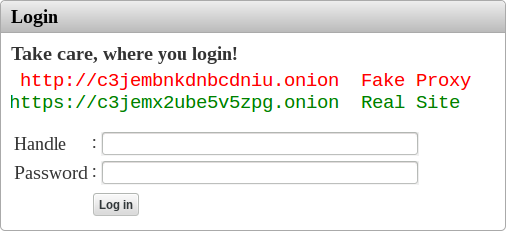
\includegraphics[width=0.7\linewidth]{figures/login-warning-1.png}
    \caption{During the login process, an onion site explicitly warns of an
    impersonation site.}
    \label{fig:login-warning-1}
  \end{subfigure}

  \begin{subfigure}[b]{\linewidth}
    \centering
    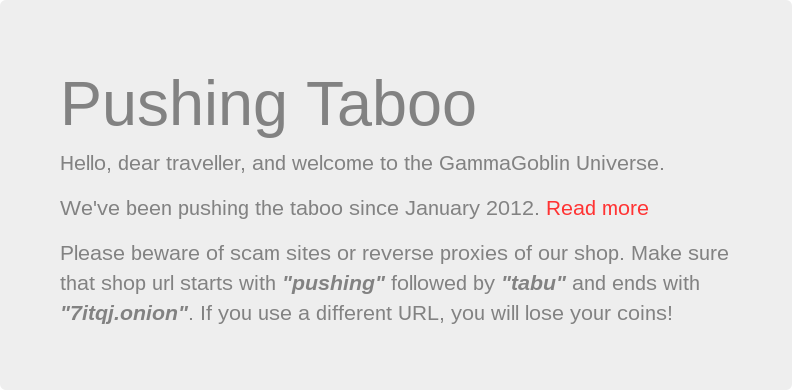
\includegraphics[width=0.8\linewidth]{figures/login-warning-2.png}
    \caption{Aware of an ongoing phishing attack, another onion site warns its
    users of impersonation sites.}
    \label{fig:login-warning-2}
  \end{subfigure}

  \caption{Reacting to phishing attacks, some onion service operators now
  display warnings as part of the login process.}
\end{figure}

Possible to use scallion~\cite{scallion}.

In practice, most naming schemes only seem to satisfy two out of these three
properties.  This observation is colloquially referred to as ``Zooko's
triangle,'' illustrated in \autoref{fig:naming-triangle}.  DNS is memorable
and global but not secure because numerous attacks exist to feed DNS users a
false mapping from domain to IP address.  Onion domains are secure and global
but not memorable because they are long and randomly generated.  Petname systems
(e.g., your buddy list in your instant messaging application) are memorable and
secure but not global.

\begin{figure}
\centering
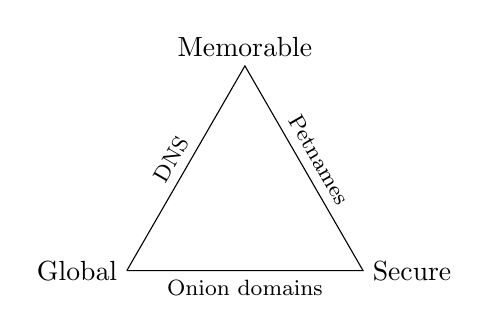
\begin{tikzpicture}

\draw (0.0,0.0) node[anchor=east] {Global}
        -- node [midway, below, sloped] {{\footnotesize Onion domains}}
      (3.0,0.0) node[anchor=west] {Secure}
        -- node [midway, above, sloped] {{\footnotesize Petnames}}
      (1.5,2.6) node[anchor=south] {Memorable}
        -- node [midway, above, sloped] {{\footnotesize DNS}}
      (0.0,0.0);

\end{tikzpicture}
\caption{``Zooko's triangle,'' a conjecture that posits that any naming scheme
can only satisfy two properties out of secure, memorable, and global.}
\label{fig:naming-triangle}
\end{figure}


\section{Survey design}
\label{sec:survey-design}

We investigate how Tor users interact with onion services by designing and
administering a survey.

\subsection{Research question}
We designed the survey to answer the following research questions: \emph{How do
Tor users interact with onion services?}  An answer to this research question
allows us to both create more usable anonymity systems and build these systems
in a way that human-centered attacks such as phishing are exacerbated.  In
particular, we seek to answer the following three aspects:

\begin{itemize}
    \item What is the expectation of privacy when people use Tor Browser in
        general and onion sites in particular?
    \item What is the security/usability trade-off of vanity onion domains?
    \item Do people handle onion domains differently than normal domains?
\end{itemize}

\subsection{Design}
\begin{itemize}
    \item Our survey consists of six blocks:
        \begin{enumerate}
            \item Consent and demographics
            \item Tor usage
            \item Onion site usage
            \item Onion site operation
            \item Onion site phishing and impersonation
            \item Expectations of privacy
        \end{enumerate}
    \item Mention that we got IRB approval once we got it.
    \item We implemented our survey in Qualtrics and made sure that it can be
        answered correctly over Tor Browser.  Used a Qualtrics feature so that
        participants can answer the survey only once.
    \item We used four screener questions distributed over four distinct
        blocks, \ie, questions whose sole purpose is to check whether the
        respondent is paying attention.~\cite{Berinsky2014a}.
    \item Having followed mailing lists \etc for many years, we did not feel the
        need for focus groups to explore what topics are worth inquiring.
    \item Used cognitive pretesting (sometimes also called cognitive
        interviewing)~\cite{Collins2003a}.  Pretesting can show us that
        respondents \first understand questions, \second understand questions
        consistently, and \third understand questions the way that we intended.
        Two main strategies are \emph{think-aloud interviewing} and
        \emph{probing}.  In addition, we can ask respondends about the
        confidence they have in their responses.  However, not all cognitive
        processes can be verbalized and cognitive pretesting may change the way
        respondents answer questions.  We had $N$ respondents (talk about
        demographics) based on whose input we iteratively improved our survey.

        $M$ respondents were fluent, but non-native English speakers.
    \item We tried hard to have neutral, non-leading questions.
    \item Question randomization.
    \item Basic statistics.  The survey consists of X questions and takes
        approximately Y minutes to complete.  We used our university's
        Qualtrics membership to create the survey.
\end{itemize}

\subsection{Participant recruiting}
\begin{itemize}
    \item Tor's population is unknown.  We barely know its size.  Besides, there
        is no way to recruit all Tor users with equal probability.  Therefore,
        we will have inevitable sampling bias in our results.  We work around
        that by using diverse recruitment media and making our sample size as
        large as possible.
    \item Post on Tor's blog?\\\url{https://blog.torproject.org}
    \item Ask Tor to post on its Twitter account?\\\url{https://twitter.com/torproject}
    \item Post on Tor's mailing lists
    \item Post on social media such as:
        \begin{itemize}
            \item \url{https://reddit.com/r/tor/}
            \item \url{https://reddit.com/r/onions/}
            \item \url{https://reddit.com/r/samplesize/}
        \end{itemize}
    \item Use Amazon's Mechanical Turk
    \item Facebook ads?
    \item Google surveys?
    \item Craigslist?
\end{itemize}

Important things to consider in questions:
\begin{itemize}
    \item Are our results generalizable to self-authenticating names?
    \item Ordering of questions matters.
    \item Use aided recall for behavioral questions.
    \item Questions should be non-threatening (is there a ``right'' or ``wrong''
        answer?).  If respondents think they would
        look bad, they may answer not truthfully.
    \item Avoid jargon and unusual vocabulary (to non-native English speakers)
\end{itemize}

\subsection{Incentives for participation}
\begin{itemize}
    \item Have a few high-value gift cards in lottery.
    \item Have many low-value gift cards for everyone.
    \item Bitcoins?
\end{itemize}

\subsection{Data analysis}

\subsection{Limitations}
\begin{itemize}
    \item Representative sample?
\end{itemize}


\section{Results}
\label{sec:results}

\subsection{Participants}
\begin{itemize}
    \item Provide intuition on how much our sample resembles the general
        population.
    \item From when to when did we disseminate our survey?
    \item How many participants did we attract?
    \item How long did it take to complete the survey?  Provide some descriptive statistics.
    \item What's the female/male ratio?
    \item What's the age distribution?
    \item What's the level of education?
    \item What's the computer security knowledge?  Note that our participants
        may overestimate their knowledge.
\end{itemize}

\subsection{Random anecdotes}
\begin{itemize}
    \item In pre-test: one person considered the onion domain itself
        confidential and was worried about the domain's prefix revealing
        anything about its content.
\end{itemize}


\section{Discussion}
\label{sec:discussion}

\begin{itemize}
    \item Tor is working on a new onion service design~\cite{Mathewson2013a}.
        Anything we can say about that?
\end{itemize}

\subsection{Limitations}
\begin{itemize}
    \item Our demographic may not be representative because we selected people
        who may care more about onion sites than the average Tor user.  Many
        Tor users may do nothing other than download Tor Browser.
    \item Our survey was only in English, so it may not generalize well to
        non-English speakers.  We know that there are cultural differences in
        security behavior~\cite{Sawaya2017a}.
\end{itemize}


\section{Conclusion}
\label{sec:conclusion}


\section*{Acknowledgements}
We want to thank George Kadianakis for helpful feedback.

We want to thank Laura M. Roberts, Roya Ensafi, Will Scott, and Jens Kubiziel
for help with pre-testing the survey.

Thanks to Katherine Haenschen for helping us improve our method.

This research was supported in part by the Center for Information Technology
Policy at Princeton University.  This project was further supported in part by
National Science Foundation Awards CNS-1540055 and CNS-1602399.


\balance
\printbibliography

\appendix

\section{Pre-interview survey}
\label{app:interview-survey}
We asked potential interview subjects to fill out a short survey (see below)
before we proceeded with selecting our subjects.  This survey allowed us to
select for subjects with the most interesting background.

\begin{enumerate}
    \item What is your name?
    \item What is your email address?
    \item Are you 18 years or older?
        \begin{itemize}[label=$\Circle$]
            \item Yes
            \item No
        \end{itemize}
    \item Have you used Tor Browser in the past?
        \begin{itemize}[label=$\Circle$]
            \item Yes
            \item No
        \end{itemize}
    \item Have you used onion services in the past?
        \begin{itemize}[label=$\Circle$]
            \item Yes
            \item No
        \end{itemize}
    \item How do you rate your knowledge about Internet privacy and security?
        \begin{itemize}[label=$\Circle$]
            \item Not at all knowledgeable
            \item Slightly knowledgeable
            \item Somewhat knowledgeable
            \item Moderately knowledgeable
            \item Extremely knowledgeable
        \end{itemize}
\end{enumerate}

\section{Interview questions}
\label{app:interview-questions}

We started the interview by handing our interviewees the consent form and
explained the purpose of our research to them.

\paragraph{Introductory questions}
\begin{enumerate}
    \item Tell us how often and why you use Tor?
    \item Do you remember the first time you used Tor?
\end{enumerate}

\paragraph{Expectations of privacy}
\begin{enumerate}
    \item What would make you use onion services more? (speed, quality/quantity
        of content, better domain format, popular websites having onion sites)
    \item Who or what are you trying to protect yourself against when using Tor?
    \item The domain format of onion sites is weird.  How do you deal with that?
    \item Would you like it if Tor Browser automatically redirected you to onion
        sites?  Even if that were the case for all onion sites?
    \item How do you learn about new onion sites?
    \item Do you think phishing is a concern with onion sites?  How do you know
        if an onion site is legitimate?
    \item Assume you use Tor to open \texttt{example.com}.  Who can see what?
        What if you open the corresponding onion site instead?
    \item What are you concerned about when using Tor?
    \item Certain things are hidden from certain entities when you are using
        Tor.  Please explain your beliefs.
    \item Some websites use ``vanity onion domains.''  Whare are your thoughts
        on that?
    \item Explain in your own words how you believe Tor works.
    \item Is there anything else about the usability of onion services that you
        wish to share?
\end{enumerate}

\section{Survey questions}
This section contains our online survey, consisting of seven sections.  Each
section holds a number of questions and their respective responses.  In the
responses, circles indicate that only one response can be selected while squares
indicate the possibility to select multiple responses.

\subsection{Demographic information}
\begin{enumerate}
    \item What is your gender?
        \begin{itemize}[label=$\Circle$]
            \item Female
            \item Male
            \item Other
        \end{itemize}

    \item What is your age?
        \begin{itemize}[label=$\Circle$]
            \item 18--25 years
            \item 26--35 years
            \item 36--45 years
            \item 46-55 years
            \item 56--65 years
            \item Older than 65 years
        \end{itemize}

    \item What is the highest level of education that you completed?
        \begin{itemize}[label=$\Circle$]
            \item Some education, but no high school diploma or equivalent
            \item High school diploma or equivalent
            \item College or university degree (for example a bachelor's degree)
            \item Post-graduate education (for example a master's or a doctorate degree)
        \end{itemize}

    \item How would you rate your knowledge about Internet privacy and security?
        \begin{itemize}[label=$\Circle$]
            \item No knowledge
            \item Mildly knowledgeable
            \item Moderately knowledgeable
            \item Highly knowledgeable
            \item Expert
        \end{itemize}
\end{enumerate}

\subsection{Tor usage}
\begin{enumerate}
    \item Tor Browser is a web browser---similar to Firefox---that allows you
        to browse the web anonymously. Have you ever used Tor Browser?
        \begin{itemize}[label=$\Circle$]
            \item Yes
            \item No
        \end{itemize}

    \item How frequently do you use Tor Browser?\\(Please select the answer
        that applies the most.)
        \begin{itemize}[label=$\Circle$]
            \item Never
            \item On average less than once a month
            \item On average about once a month
            \item On average about once a week
            \item On average about once a day
            \item Tor Browser is my main browser
        \end{itemize}

    \item When using Tor Browser, who do you want to protect your browsing
        activity from?\\(Check all that apply.)
        \begin{itemize}[label=$\Square$]
            \item My government
            \item Other governments
            \item My Internet service provider (ISP)
            \item My school
            \item My employer
            \item Friends and family
            \item Advertising companies
            \item Hackers in open WiFis (for example in coffee shops)
            \item Other (Please elaborate below.)
        \end{itemize}

    \item For quality purposes, please select only ``iPhone'' and ``Android''
        in the options below.
        \begin{itemize}[label=$\Square$]
            \item PC
            \item Mac
            \item iPhone
            \item Android
            \item Other (Please elaborate below.)
        \end{itemize}
\end{enumerate}

\subsection{Onion site usage}
\begin{enumerate}
    \item The Tor Browser allows you to browse ``onion sites.'' Onion sites are
        web sites that can only be accessed over the Tor network. The domains of
        onion sites end with \texttt{.onion} instead of \texttt{.com},
        \texttt{.net}, etc.; they are of constant length; and they tend to
        ``look random.'' For example, The Tor Project's web site,
        \texttt{torproject.org}, is also available at
        \texttt{expyuzz4wqqyqhjn.onion} as an onion site.

    \item How frequently do you use Tor Browser to browse onion sites?\\(Please
        select the answer that applies the most.)
        \begin{itemize}[label=$\Circle$]
            \item I have never used onion sites
            \item On average less than once a month
            \item On average about once a month
            \item On average about once a week
            \item On average about once a day
        \end{itemize}

    \item How frequently do you use onion sites for purposes other than web
        browsing? For example for remote login (SSH) or chat (IRC, or XMPP)?
        \begin{itemize}[label=$\Circle$]
            \item Never
            \item On average less than once a month
            \item On average about once a month
            \item On average about once a week
            \item On average about once a day
        \end{itemize}

    \item Why do you browse onion sites?\\(Check all that apply.)
        \begin{itemize}[label=$\Square$]
            \item Because of the additional anonymity -- traffic to onion sites
                never leaves the Tor network
            \item Because of the additional security -- onion sites provide
                end-to-end security
            \item Some sites I like are only available as onion sites and not
                as normal web sites
            \item No particular reason; I occasionally just click on links to
                onion sites
            \item I read about the ``dark web'' and wanted to form my own
                opinion
            \item Other (Please elaborate below.)
        \end{itemize}

    \item How do you discover new onion sites?\\(Check all that apply.)
        \begin{itemize}[label=$\Square$]
            \item I browse the list of onion site search engines such as
                \texttt{ahmia.fi}
            \item From social networking sites such as Reddit or Twitter
            \item Recommendations from friends and family
            \item I randomly encounter them while browsing the web
            \item I am not interested in learning about new onion sites
            \item Other (Please elaborate below.)
        \end{itemize}

    \item Are you satisfied with the way you discover new onion sites?\\(Check
        all that apply.)
        \begin{itemize}[label=$\Circle$]
            \item Yes
            \item No (Please elaborate below.)
        \end{itemize}

    \item Many people memorize popular domains such as \texttt{youtube.com} and
        \texttt{wikipedia.com} for quick access. How do you deal with the domain
        of onion sites such as \texttt{expyuzz4wqqyqhjn.onion}?\\(Check all that
        apply.)
        \begin{itemize}[label=$\Square$]
            \item I save a list of onion domains in a file on my computer
            \item I write onion domains down using pen and paper
            \item I bookmark onion domains in Tor Browser
            \item I use a web-based bookmarking service such as Firefox Sync or
                Google Bookmarks
            \item I use a search engine each time (for example, to search for
                ``facebook onion site'')
            \item I go to web pages I trust that have links to onion sites
            \item I memorize some onion domains
            \item I don't have a good solution
            \item Other (Please elaborate below.)
        \end{itemize}

    \item The Tor Project is currently working on the next generation of onion
        services. The new onion domain format will consist of 52 characters,
        for example:
        \texttt{a1uik0w1gmfq3i5ievxdm9ceu27e88g6o7pe0rffdw9jmn\-twkdsd.onion}
        Do you expect this to change your browsing habits?
        \begin{itemize}[label=$\Circle$]
            \item Yes (Please elaborate below.)
            \item No (Please elaborate below.)
        \end{itemize}

    \item Do you have a Facebook account?
        \begin{itemize}[label=$\Circle$]
            \item Yes
            \item No
        \end{itemize}

    \item Have you ever logged in to Facebook over its onion site
        \texttt{facebookcorewwwi.onion}?
        \begin{itemize}[label=$\Circle$]
            \item Yes, that is the only way I log in to Facebook
            \item Yes, occasionally
            \item No, never
            \item I didn't know about this onion site until now
        \end{itemize}

    \item For quality purposes, please select ``Yes, more than once'' in the
        options below.
        \begin{itemize}[label=$\Circle$]
            \item Yes, once
            \item Yes, more than once
            \item No
        \end{itemize}

    \item How many onion domains do you have fully memorized?
        \begin{itemize}[label=$\Circle$]
            \item None
            \item One
            \item Two
            \item Three
            \item Four
            \item More than four
        \end{itemize}

    \item Is \texttt{facebookcorewwwi.onion} among the sites that you have
        memorized?
        \begin{itemize}[label=$\Circle$]
            \item Yes
            \item No
        \end{itemize}

    \item Why do you memorize onion domains?\\(Check all that apply.)
        \begin{itemize}[label=$\Square$]
            \item It allows me to open the site more quickly
            \item I don't want to leave any digital traces of the onion sites I
                visit
            \item That way I can be sure that I end up at the right onion site
                and not a phishing site
            \item After typing a domain many times, I automatically start to
                memorize it
            \item Other (Please elaborate below.)
        \end{itemize}

    \item Imagine you had to memorize onion domains. Please rate the difficulty
        of memorizing the following domains.
        \begin{itemize}
            \item \texttt{facebookcorewwwi.onion}
            \item \texttt{expyuzz4wqqyqhjn.onion}
            \item \texttt{torproz4wqqyqhjn.onion}
            \item \texttt{torprojectqyqhjn.onion}
        \end{itemize}
        For each answer, we provided the following Likert scale:
        \begin{itemize}
            \item Very easy
            \item Somewhat easy
            \item Neither easy nor difficult
            \item Somewhat difficult
            \item Very difficult
        \end{itemize}

    \item Please explain the reason for the rating you gave above.

    \item If popular web sites such as YouTube, Twitter, or Amazon offered
        onion sites in parallel to their normal web sites, which one would you
        prefer?
        \begin{itemize}[label=$\Circle$]
            \item Always the normal web site
            \item Always the onion site
            \item Other (Please elaborate below.)
        \end{itemize}

    \item Please explain the reason for the choice you made above.

    \item If Tor Browser could automatically redirect you from a web site to
        its corresponding onion site (for example from \texttt{facebook.com} to
        \texttt{facebookcorewwwi.onion}), would you use this feature?
        \begin{itemize}[label=$\Circle$]
            \item No, never
            \item Yes, for some sites
            \item Yes, always
            \item Other (Please elaborate below.)
        \end{itemize}

    \item Please explain the reason for the choice you made above.

    \item Please rate how important the following criteria are for the
        usability of onion sites.\\(Check all that apply.)
        \begin{itemize}
            \item Page load time
            \item Quality of content (e.g., up-to-date, interesting sites)
            \item Diversity of content (e.g., sites about politics, technology, social media, etc.)
            \item Easy-to-remember domain format
            \item Having an onion service version of popular services such as Facebook
            \item Existence of a search engine (like Google) for onion services
        \end{itemize}
        For each answer, we provided the following Likert scale:
        \begin{itemize}
            \item Very unimportant
            \item Somewhat unimportant
            \item Neutral
            \item Somewhat important
            \item Very important
        \end{itemize}
\end{enumerate}

\subsection{Onion site operation}
\begin{enumerate}
    \item Have you ever set up your own onion site?
        \begin{itemize}[label=$\Circle$]
            \item Yes
            \item No, but I have considered doing it
            \item No, and I have not considered it
        \end{itemize}

    \item Did you experience any issues while setting up your onion site?
        \begin{itemize}[label=$\Circle$]
            \item No
            \item Yes (Please elaborate below.)
        \end{itemize}

    \item Why did you set up your own onion site?\\(Check all that apply.)
        \begin{itemize}[label=$\Square$]
            \item I wanted my site to be anonymous
            \item I wanted my site to have end-to-end security
            \item I used a tool that automatically creates onion sites (for
                example OnionShare or Ricochet)
            \item To make my site accessible behind a NAT device
            \item Out of curiosity
            \item Other (Please elaborate below.)
        \end{itemize}

    \item Were the onion site(s) you set up intended for the general public, or
        only for private use?\\(Check all that apply.)
        \begin{itemize}[label=$\Square$]
            \item For public use (for example, a public blog)
            \item For private use (for example, sharing pictures with a friend)
        \end{itemize}

    \item Please rate the level of concern you would have for the following
        scenarios.
        \begin{itemize}
            \item Somebody deanonymizing my onion service
            \item Somebody taking my onion service offline
            \item Somebody setting up a phishing site targeting my onion service
        \end{itemize}
        For each answer, we provided the following Likert scale:
        \begin{itemize}
            \item Not at all concerned
            \item Slightly concerned
            \item Somewhat concerned
            \item Moderately concerned
            \item Extremely concerned
        \end{itemize}
\end{enumerate}

\subsection{Onion site phishing and impersonation}
\begin{enumerate}
    \item Did you ever type an onion domain manually?
        \begin{itemize}[label=$\Circle$]
            \item Yes
            \item No
        \end{itemize}

    \item Please elaborate on why you typed an onion domain manually?

    \item How do you realize that you made a typo when typing an onion
        URL?\\(Check all that apply.)
        \begin{itemize}[label=$\Square$]
            \item When the page won't load
            \item When a wrong page shows up
            \item I don't know
            \item Other (Please elaborate below.)
        \end{itemize}

    \item Have you ever thought about whether the onion site you are browsing
        is the authentic site you are trying to reach?
        \begin{itemize}[label=$\Circle$]
            \item Yes
            \item No
        \end{itemize}

    \item How do you know an onion site is the legitimate site you are trying
        to reach, and not an impersonation?\\(Check all that apply.)
        \begin{itemize}[label=$\Square$]
            \item I verify (part of) the onion domain in Tor Browser's address
                bar
            \item I use bookmarks when accessing onion sites
            \item I go to the corresponding web site and look for the link to
                its onion site
            \item Sometimes I cannot tell the difference between the legitimate
                and the impersonation site
            \item I copy\&paste onion domains from a trusted source
            \item I check if the onion site's HTTPS certificate is valid (if it
                has one)
            \item I don't check
            \item Other (Please elaborate below.)
        \end{itemize}

    \item How many characters of a domain do you verify? Recall that an onion
        domain has 16 characters.
        \begin{itemize}[label=$\Circle$]
            \item 1--3
            \item 4--6
            \item 7--9
            \item 10--12
            \item 13--16
        \end{itemize}

    \item For quality purposes, please select ``Less than once a month'' in the
        options below.
        \begin{itemize}[label=$\Circle$]
            \item Less than once a month
            \item About once a month
            \item About once a week
            \item About once a day
        \end{itemize}

    \item Have you ever sent Bitcoins to a Bitcoin address that you got from an
        onion site?
        \begin{itemize}[label=$\Circle$]
            \item Yes
            \item No
        \end{itemize}

    \item Some onion site owners use tools to have a short word at the
        beginning of their onion domain. This is why Facebook's domain
        (\texttt{facebookcorewwwi.onion}) looks the way it does. We call these
        customized domains ``vanity onion domains.''

    \item What is your overall opinion on vanity onion domains?\\(Check all
        that apply.)
        \begin{itemize}[label=$\Square$]
            \item I find them useful because they are easier to memorize
            \item I find them useful because they are easier to recognize
            \item I like them because they make an onion site look ``unique''
            \item I dislike them because onion sites shouldn't contain their
                name in their domain
            \item I don't see a benefit
            \item I don't have an opinion
            \item Other (Please elaborate below.)
        \end{itemize}
\end{enumerate}

\subsection{Expectations of privacy}
\begin{enumerate}
    \item Let us move away from onion services and turn to expectations of
        privacy. If you use Tor Browser to open \texttt{http://example.com}, who
        do you believe can see your connection to
        \texttt{http://example.com}?\\(Check all that apply.)
        \begin{itemize}[label=$\Square$]
            \item Your Internet service provider (ISP)
            \item The ISP of \texttt{example.com}
            \item Your Tor ``exit relay''
            \item Your Tor ``guard relay''
            \item Nobody
            \item I don't know
            \item Other (Please elaborate below.)
        \end{itemize}

    \item Now imagine that you are instead using Tor Browser to open the
        \emph{onion site} of \texttt{http://example.com}. Who do you believe can
        see your connection to this onion site?\\(Check all that apply.)
        \begin{itemize}[label=$\Square$]
            \item Your Internet service provider (ISP)
            \item The ISP of the onion site
            \item Your Tor ``exit relay''
            \item Your Tor ``guard relay''
            \item The ``guard relay'' of the onion site
            \item Nobody
            \item I don't know
            \item Other (Please elaborate below.)
        \end{itemize}

    \item How safe do you feel when using Tor Browser compared to another
        browser?
        \begin{itemize}[label=$\Circle$]
            \item Very unsafe
            \item Somewhat unsafe
            \item Neutral
            \item Somewhat safe
            \item Very safe
        \end{itemize}

    \item Please elaborate on why you feel that way when using Tor Browser.

    \item Please tell us about how safe you feel when browing onion sites as
        compared to normal websites?
        \begin{itemize}[label=$\Circle$]
            \item Very unsafe
            \item Somewhat unsafe
            \item Neutral
            \item Somewhat safe
            \item Very safe
        \end{itemize}

    \item Please elaborate on why you feel that way when using onion sites.

    \item For quality purposes, please select only ``Very unsafe'' in the options
        below.
        \begin{itemize}[label=$\Circle$]
            \item Very unsafe
            \item Somewhat unsafe
            \item Neutral
            \item Somewhat safe
            \item Very safe
        \end{itemize}

    \item Assume you just set up your own onion site. Who do you believe can
        see that this onion site was set up?\\(Check all that apply.)
        \begin{itemize}[label=$\Square$]
            \item The onion site's ISP
            \item The developers of The Tor Project
            \item (Some) Tor relays
            \item Nobody
            \item I don't know
            \item Other (Please elaborate below.)
        \end{itemize}

    \item Facebook already runs the onion site \texttt{facebookcorewwwi.onion}.
        How difficult or easy do you believe is it for someone to create domains
        that begin with the following characters? Note that the {\color{red}
        \texttt{X}} symbols below
        are just placeholders. What matters is the first characters.
        \begin{itemize}
            \item \texttt{facebookcore\textcolor{red}{XXXX}.onion}
            \item \texttt{facebook\textcolor{red}{XXXXXXXX}.onion}
            \item \texttt{face\textcolor{red}{XXXXXXXXXXXX}.onion}
        \end{itemize}
        For each answer, we provided the following Likert scale:
        \begin{itemize}
            \item Very easy
            \item Moderately easy
            \item Neither easy nor difficult
            \item Moderately difficult
            \item Very difficult
            \item I don't know
        \end{itemize}
\end{enumerate}

\subsection{End of survey}
\begin{enumerate}
    \item Finally, is there anything else about the usability of Tor or onion
        services that you wish to share with us?
\end{enumerate}


\end{document}
